\subsubsection{} \textit{AES} шифровка и расшифровка.
\label{sec:eng:performance:aesenc}

Завершающей парой тестовых методов являются методы для шифровки и расшифровки при помощи алгоритма \textit{AES}: \texttt{aesEncrypt} и \texttt{aesDecrypt}. На рисунках \ref{sec:eng:performance:aesenc:enc} и \ref{sec:eng:performance:aesenc:dec} результаты измерений генерации \textit{RSA} и \textit{AES} ключей соответственно.

\begin{figure}[h]
\centering
\begin{minipage}{.5\textwidth}
  \centering
  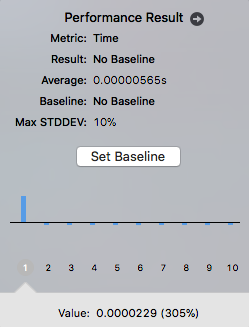
\includegraphics[width=.65\linewidth]{inc/img/perf/testAESEncryptPerformance.png}
  \captionof{figure}{Результаты замеров шифровки при помощи AES}
  \label{sec:eng:performance:aesenc:enc}
\end{minipage}%
\begin{minipage}{.5\textwidth}
  \centering
  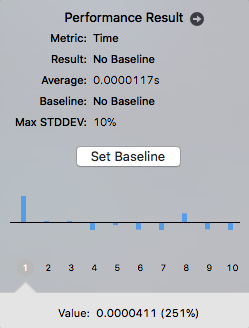
\includegraphics[width=.65\linewidth]{inc/img/perf/testAESDecryptPerformance.png}
  \captionof{figure}{Результаты замеров дешифровки при помощи AES}
  \label{sec:eng:performance:aesenc:dec}
\end{minipage}
\end{figure}